\documentclass[12pt,a4paper]{article}

\usepackage[a4paper,width=160mm,top=25mm,bottom=25mm]{geometry}

\usepackage{fancyhdr}
\pagestyle{fancy}
\fancyhf{}
\fancyhead[EL]{\nouppercase\leftmark}
\fancyhead[OR]{\nouppercase\rightmark}
\fancyhead[ER,OL]{\thepage}

\usepackage{url}
\usepackage[hidelinks]{hyperref}

\renewcommand{\linethickness}{0.05em}
\usepackage[brazil]{babel}   
\usepackage{titlesec}
\newcommand{\sectionbreak}{\clearpage}


\title{Processando a Informação: um livro prático de programação independente de linguagem 
\\\large\vspace{2cm}
Rogério Perino de Oliveira Neves 
\\\vspace{5mm}
Francisco de Assis Zampirolli
\\\large\vspace{2cm}
EDUFABC
\\ \url{editora.ufabc.edu.br}
\\\Huge\vspace{3cm}
Notas de Aulas inspiradas no livro
\\\Large\vspace{1cm}
Utilizando a(s) Linguagem(ns) de Programação: 
\\\Huge\vspace{1cm}
C
\\\large\vspace{1cm}
Exemplos adaptados para Correção Automática no Moodle+VPL
\vspace{2cm}}
\author{Francisco de Assis Zampirolli\vspace{1cm}}


    \usepackage[breakable]{tcolorbox}
    \usepackage{parskip} % Stop auto-indenting (to mimic markdown behaviour)
    

    % Basic figure setup, for now with no caption control since it's done
    % automatically by Pandoc (which extracts ![](path) syntax from Markdown).
    \usepackage{graphicx}
    % Maintain compatibility with old templates. Remove in nbconvert 6.0
    \let\Oldincludegraphics\includegraphics
    % Ensure that by default, figures have no caption (until we provide a
    % proper Figure object with a Caption API and a way to capture that
    % in the conversion process - todo).
    \usepackage{caption}
    \DeclareCaptionFormat{nocaption}{}
    \captionsetup{format=nocaption,aboveskip=0pt,belowskip=0pt}

    \usepackage{float}
    \floatplacement{figure}{H} % forces figures to be placed at the correct location
    \usepackage{xcolor} % Allow colors to be defined
    \usepackage{enumerate} % Needed for markdown enumerations to work
    \usepackage{geometry} % Used to adjust the document margins
    \usepackage{amsmath} % Equations
    \usepackage{amssymb} % Equations
    \usepackage{textcomp} % defines textquotesingle
    % Hack from http://tex.stackexchange.com/a/47451/13684:
    \AtBeginDocument{%
        \def\PYZsq{\textquotesingle}% Upright quotes in Pygmentized code
    }
    \usepackage{upquote} % Upright quotes for verbatim code
    \usepackage{eurosym} % defines \euro

    \usepackage{iftex}
    \ifPDFTeX
        \usepackage[T1]{fontenc}
        \IfFileExists{alphabeta.sty}{
              \usepackage{alphabeta}
          }{
              \usepackage[mathletters]{ucs}
              \usepackage[utf8x]{inputenc}
          }
    \else
        \usepackage{fontspec}
        \usepackage{unicode-math}
    \fi

    \usepackage{fancyvrb} % verbatim replacement that allows latex
    \usepackage{grffile} % extends the file name processing of package graphics
                         % to support a larger range
    \makeatletter % fix for old versions of grffile with XeLaTeX
    \@ifpackagelater{grffile}{2019/11/01}
    {
      % Do nothing on new versions
    }
    {
      \def\Gread@@xetex#1{%
        \IfFileExists{"\Gin@base".bb}%
        {\Gread@eps{\Gin@base.bb}}%
        {\Gread@@xetex@aux#1}%
      }
    }
    \makeatother
    \usepackage[Export]{adjustbox} % Used to constrain images to a maximum size
    \adjustboxset{max size={0.9\linewidth}{0.9\paperheight}}

    % The hyperref package gives us a pdf with properly built
    % internal navigation ('pdf bookmarks' for the table of contents,
    % internal cross-reference links, web links for URLs, etc.)
    \usepackage{hyperref}
    % The default LaTeX title has an obnoxious amount of whitespace. By default,
    % titling removes some of it. It also provides customization options.
    \usepackage{titling}
    \usepackage{longtable} % longtable support required by pandoc >1.10
    \usepackage{booktabs}  % table support for pandoc > 1.12.2
    \usepackage{array}     % table support for pandoc >= 2.11.3
    \usepackage{calc}      % table minipage width calculation for pandoc >= 2.11.1
    \usepackage[inline]{enumitem} % IRkernel/repr support (it uses the enumerate* environment)
    \usepackage[normalem]{ulem} % ulem is needed to support strikethroughs (\sout)
                                % normalem makes italics be italics, not underlines
    \usepackage{mathrsfs}
    

    
    % Colors for the hyperref package
    \definecolor{urlcolor}{rgb}{0,.145,.698}
    \definecolor{linkcolor}{rgb}{.71,0.21,0.01}
    \definecolor{citecolor}{rgb}{.12,.54,.11}

    % ANSI colors
    \definecolor{ansi-black}{HTML}{3E424D}
    \definecolor{ansi-black-intense}{HTML}{282C36}
    \definecolor{ansi-red}{HTML}{E75C58}
    \definecolor{ansi-red-intense}{HTML}{B22B31}
    \definecolor{ansi-green}{HTML}{00A250}
    \definecolor{ansi-green-intense}{HTML}{007427}
    \definecolor{ansi-yellow}{HTML}{DDB62B}
    \definecolor{ansi-yellow-intense}{HTML}{B27D12}
    \definecolor{ansi-blue}{HTML}{208FFB}
    \definecolor{ansi-blue-intense}{HTML}{0065CA}
    \definecolor{ansi-magenta}{HTML}{D160C4}
    \definecolor{ansi-magenta-intense}{HTML}{A03196}
    \definecolor{ansi-cyan}{HTML}{60C6C8}
    \definecolor{ansi-cyan-intense}{HTML}{258F8F}
    \definecolor{ansi-white}{HTML}{C5C1B4}
    \definecolor{ansi-white-intense}{HTML}{A1A6B2}
    \definecolor{ansi-default-inverse-fg}{HTML}{FFFFFF}
    \definecolor{ansi-default-inverse-bg}{HTML}{000000}

    % common color for the border for error outputs.
    \definecolor{outerrorbackground}{HTML}{FFDFDF}

    % commands and environments needed by pandoc snippets
    % extracted from the output of `pandoc -s`
    \providecommand{\tightlist}{%
      \setlength{\itemsep}{0pt}\setlength{\parskip}{0pt}}
    \DefineVerbatimEnvironment{Highlighting}{Verbatim}{commandchars=\\\{\}}
    % Add ',fontsize=\small' for more characters per line
    \newenvironment{Shaded}{}{}
    \newcommand{\KeywordTok}[1]{\textcolor[rgb]{0.00,0.44,0.13}{\textbf{{#1}}}}
    \newcommand{\DataTypeTok}[1]{\textcolor[rgb]{0.56,0.13,0.00}{{#1}}}
    \newcommand{\DecValTok}[1]{\textcolor[rgb]{0.25,0.63,0.44}{{#1}}}
    \newcommand{\BaseNTok}[1]{\textcolor[rgb]{0.25,0.63,0.44}{{#1}}}
    \newcommand{\FloatTok}[1]{\textcolor[rgb]{0.25,0.63,0.44}{{#1}}}
    \newcommand{\CharTok}[1]{\textcolor[rgb]{0.25,0.44,0.63}{{#1}}}
    \newcommand{\StringTok}[1]{\textcolor[rgb]{0.25,0.44,0.63}{{#1}}}
    \newcommand{\CommentTok}[1]{\textcolor[rgb]{0.38,0.63,0.69}{\textit{{#1}}}}
    \newcommand{\OtherTok}[1]{\textcolor[rgb]{0.00,0.44,0.13}{{#1}}}
    \newcommand{\AlertTok}[1]{\textcolor[rgb]{1.00,0.00,0.00}{\textbf{{#1}}}}
    \newcommand{\FunctionTok}[1]{\textcolor[rgb]{0.02,0.16,0.49}{{#1}}}
    \newcommand{\RegionMarkerTok}[1]{{#1}}
    \newcommand{\ErrorTok}[1]{\textcolor[rgb]{1.00,0.00,0.00}{\textbf{{#1}}}}
    \newcommand{\NormalTok}[1]{{#1}}

    % Additional commands for more recent versions of Pandoc
    \newcommand{\ConstantTok}[1]{\textcolor[rgb]{0.53,0.00,0.00}{{#1}}}
    \newcommand{\SpecialCharTok}[1]{\textcolor[rgb]{0.25,0.44,0.63}{{#1}}}
    \newcommand{\VerbatimStringTok}[1]{\textcolor[rgb]{0.25,0.44,0.63}{{#1}}}
    \newcommand{\SpecialStringTok}[1]{\textcolor[rgb]{0.73,0.40,0.53}{{#1}}}
    \newcommand{\ImportTok}[1]{{#1}}
    \newcommand{\DocumentationTok}[1]{\textcolor[rgb]{0.73,0.13,0.13}{\textit{{#1}}}}
    \newcommand{\AnnotationTok}[1]{\textcolor[rgb]{0.38,0.63,0.69}{\textbf{\textit{{#1}}}}}
    \newcommand{\CommentVarTok}[1]{\textcolor[rgb]{0.38,0.63,0.69}{\textbf{\textit{{#1}}}}}
    \newcommand{\VariableTok}[1]{\textcolor[rgb]{0.10,0.09,0.49}{{#1}}}
    \newcommand{\ControlFlowTok}[1]{\textcolor[rgb]{0.00,0.44,0.13}{\textbf{{#1}}}}
    \newcommand{\OperatorTok}[1]{\textcolor[rgb]{0.40,0.40,0.40}{{#1}}}
    \newcommand{\BuiltInTok}[1]{{#1}}
    \newcommand{\ExtensionTok}[1]{{#1}}
    \newcommand{\PreprocessorTok}[1]{\textcolor[rgb]{0.74,0.48,0.00}{{#1}}}
    \newcommand{\AttributeTok}[1]{\textcolor[rgb]{0.49,0.56,0.16}{{#1}}}
    \newcommand{\InformationTok}[1]{\textcolor[rgb]{0.38,0.63,0.69}{\textbf{\textit{{#1}}}}}
    \newcommand{\WarningTok}[1]{\textcolor[rgb]{0.38,0.63,0.69}{\textbf{\textit{{#1}}}}}


    % Define a nice break command that doesn't care if a line doesn't already
    % exist.
    \def\br{\hspace*{\fill} \\* }
    % Math Jax compatibility definitions
    \def\gt{>}
    \def\lt{<}
    \let\Oldtex\TeX
    \let\Oldlatex\LaTeX
    \renewcommand{\TeX}{\textrm{\Oldtex}}
    \renewcommand{\LaTeX}{\textrm{\Oldlatex}}
    % Document parameters
    % Document title
    %\title{cap4.part1.c}
    
    
    
    
    
% Pygments definitions
\makeatletter
\def\PY@reset{\let\PY@it=\relax \let\PY@bf=\relax%
    \let\PY@ul=\relax \let\PY@tc=\relax%
    \let\PY@bc=\relax \let\PY@ff=\relax}
\def\PY@tok#1{\csname PY@tok@#1\endcsname}
\def\PY@toks#1+{\ifx\relax#1\empty\else%
    \PY@tok{#1}\expandafter\PY@toks\fi}
\def\PY@do#1{\PY@bc{\PY@tc{\PY@ul{%
    \PY@it{\PY@bf{\PY@ff{#1}}}}}}}
\def\PY#1#2{\PY@reset\PY@toks#1+\relax+\PY@do{#2}}

\@namedef{PY@tok@w}{\def\PY@tc##1{\textcolor[rgb]{0.73,0.73,0.73}{##1}}}
\@namedef{PY@tok@c}{\let\PY@it=\textit\def\PY@tc##1{\textcolor[rgb]{0.24,0.48,0.48}{##1}}}
\@namedef{PY@tok@cp}{\def\PY@tc##1{\textcolor[rgb]{0.61,0.40,0.00}{##1}}}
\@namedef{PY@tok@k}{\let\PY@bf=\textbf\def\PY@tc##1{\textcolor[rgb]{0.00,0.50,0.00}{##1}}}
\@namedef{PY@tok@kp}{\def\PY@tc##1{\textcolor[rgb]{0.00,0.50,0.00}{##1}}}
\@namedef{PY@tok@kt}{\def\PY@tc##1{\textcolor[rgb]{0.69,0.00,0.25}{##1}}}
\@namedef{PY@tok@o}{\def\PY@tc##1{\textcolor[rgb]{0.40,0.40,0.40}{##1}}}
\@namedef{PY@tok@ow}{\let\PY@bf=\textbf\def\PY@tc##1{\textcolor[rgb]{0.67,0.13,1.00}{##1}}}
\@namedef{PY@tok@nb}{\def\PY@tc##1{\textcolor[rgb]{0.00,0.50,0.00}{##1}}}
\@namedef{PY@tok@nf}{\def\PY@tc##1{\textcolor[rgb]{0.00,0.00,1.00}{##1}}}
\@namedef{PY@tok@nc}{\let\PY@bf=\textbf\def\PY@tc##1{\textcolor[rgb]{0.00,0.00,1.00}{##1}}}
\@namedef{PY@tok@nn}{\let\PY@bf=\textbf\def\PY@tc##1{\textcolor[rgb]{0.00,0.00,1.00}{##1}}}
\@namedef{PY@tok@ne}{\let\PY@bf=\textbf\def\PY@tc##1{\textcolor[rgb]{0.80,0.25,0.22}{##1}}}
\@namedef{PY@tok@nv}{\def\PY@tc##1{\textcolor[rgb]{0.10,0.09,0.49}{##1}}}
\@namedef{PY@tok@no}{\def\PY@tc##1{\textcolor[rgb]{0.53,0.00,0.00}{##1}}}
\@namedef{PY@tok@nl}{\def\PY@tc##1{\textcolor[rgb]{0.46,0.46,0.00}{##1}}}
\@namedef{PY@tok@ni}{\let\PY@bf=\textbf\def\PY@tc##1{\textcolor[rgb]{0.44,0.44,0.44}{##1}}}
\@namedef{PY@tok@na}{\def\PY@tc##1{\textcolor[rgb]{0.41,0.47,0.13}{##1}}}
\@namedef{PY@tok@nt}{\let\PY@bf=\textbf\def\PY@tc##1{\textcolor[rgb]{0.00,0.50,0.00}{##1}}}
\@namedef{PY@tok@nd}{\def\PY@tc##1{\textcolor[rgb]{0.67,0.13,1.00}{##1}}}
\@namedef{PY@tok@s}{\def\PY@tc##1{\textcolor[rgb]{0.73,0.13,0.13}{##1}}}
\@namedef{PY@tok@sd}{\let\PY@it=\textit\def\PY@tc##1{\textcolor[rgb]{0.73,0.13,0.13}{##1}}}
\@namedef{PY@tok@si}{\let\PY@bf=\textbf\def\PY@tc##1{\textcolor[rgb]{0.64,0.35,0.47}{##1}}}
\@namedef{PY@tok@se}{\let\PY@bf=\textbf\def\PY@tc##1{\textcolor[rgb]{0.67,0.36,0.12}{##1}}}
\@namedef{PY@tok@sr}{\def\PY@tc##1{\textcolor[rgb]{0.64,0.35,0.47}{##1}}}
\@namedef{PY@tok@ss}{\def\PY@tc##1{\textcolor[rgb]{0.10,0.09,0.49}{##1}}}
\@namedef{PY@tok@sx}{\def\PY@tc##1{\textcolor[rgb]{0.00,0.50,0.00}{##1}}}
\@namedef{PY@tok@m}{\def\PY@tc##1{\textcolor[rgb]{0.40,0.40,0.40}{##1}}}
\@namedef{PY@tok@gh}{\let\PY@bf=\textbf\def\PY@tc##1{\textcolor[rgb]{0.00,0.00,0.50}{##1}}}
\@namedef{PY@tok@gu}{\let\PY@bf=\textbf\def\PY@tc##1{\textcolor[rgb]{0.50,0.00,0.50}{##1}}}
\@namedef{PY@tok@gd}{\def\PY@tc##1{\textcolor[rgb]{0.63,0.00,0.00}{##1}}}
\@namedef{PY@tok@gi}{\def\PY@tc##1{\textcolor[rgb]{0.00,0.52,0.00}{##1}}}
\@namedef{PY@tok@gr}{\def\PY@tc##1{\textcolor[rgb]{0.89,0.00,0.00}{##1}}}
\@namedef{PY@tok@ge}{\let\PY@it=\textit}
\@namedef{PY@tok@gs}{\let\PY@bf=\textbf}
\@namedef{PY@tok@gp}{\let\PY@bf=\textbf\def\PY@tc##1{\textcolor[rgb]{0.00,0.00,0.50}{##1}}}
\@namedef{PY@tok@go}{\def\PY@tc##1{\textcolor[rgb]{0.44,0.44,0.44}{##1}}}
\@namedef{PY@tok@gt}{\def\PY@tc##1{\textcolor[rgb]{0.00,0.27,0.87}{##1}}}
\@namedef{PY@tok@err}{\def\PY@bc##1{{\setlength{\fboxsep}{\string -\fboxrule}\fcolorbox[rgb]{1.00,0.00,0.00}{1,1,1}{\strut ##1}}}}
\@namedef{PY@tok@kc}{\let\PY@bf=\textbf\def\PY@tc##1{\textcolor[rgb]{0.00,0.50,0.00}{##1}}}
\@namedef{PY@tok@kd}{\let\PY@bf=\textbf\def\PY@tc##1{\textcolor[rgb]{0.00,0.50,0.00}{##1}}}
\@namedef{PY@tok@kn}{\let\PY@bf=\textbf\def\PY@tc##1{\textcolor[rgb]{0.00,0.50,0.00}{##1}}}
\@namedef{PY@tok@kr}{\let\PY@bf=\textbf\def\PY@tc##1{\textcolor[rgb]{0.00,0.50,0.00}{##1}}}
\@namedef{PY@tok@bp}{\def\PY@tc##1{\textcolor[rgb]{0.00,0.50,0.00}{##1}}}
\@namedef{PY@tok@fm}{\def\PY@tc##1{\textcolor[rgb]{0.00,0.00,1.00}{##1}}}
\@namedef{PY@tok@vc}{\def\PY@tc##1{\textcolor[rgb]{0.10,0.09,0.49}{##1}}}
\@namedef{PY@tok@vg}{\def\PY@tc##1{\textcolor[rgb]{0.10,0.09,0.49}{##1}}}
\@namedef{PY@tok@vi}{\def\PY@tc##1{\textcolor[rgb]{0.10,0.09,0.49}{##1}}}
\@namedef{PY@tok@vm}{\def\PY@tc##1{\textcolor[rgb]{0.10,0.09,0.49}{##1}}}
\@namedef{PY@tok@sa}{\def\PY@tc##1{\textcolor[rgb]{0.73,0.13,0.13}{##1}}}
\@namedef{PY@tok@sb}{\def\PY@tc##1{\textcolor[rgb]{0.73,0.13,0.13}{##1}}}
\@namedef{PY@tok@sc}{\def\PY@tc##1{\textcolor[rgb]{0.73,0.13,0.13}{##1}}}
\@namedef{PY@tok@dl}{\def\PY@tc##1{\textcolor[rgb]{0.73,0.13,0.13}{##1}}}
\@namedef{PY@tok@s2}{\def\PY@tc##1{\textcolor[rgb]{0.73,0.13,0.13}{##1}}}
\@namedef{PY@tok@sh}{\def\PY@tc##1{\textcolor[rgb]{0.73,0.13,0.13}{##1}}}
\@namedef{PY@tok@s1}{\def\PY@tc##1{\textcolor[rgb]{0.73,0.13,0.13}{##1}}}
\@namedef{PY@tok@mb}{\def\PY@tc##1{\textcolor[rgb]{0.40,0.40,0.40}{##1}}}
\@namedef{PY@tok@mf}{\def\PY@tc##1{\textcolor[rgb]{0.40,0.40,0.40}{##1}}}
\@namedef{PY@tok@mh}{\def\PY@tc##1{\textcolor[rgb]{0.40,0.40,0.40}{##1}}}
\@namedef{PY@tok@mi}{\def\PY@tc##1{\textcolor[rgb]{0.40,0.40,0.40}{##1}}}
\@namedef{PY@tok@il}{\def\PY@tc##1{\textcolor[rgb]{0.40,0.40,0.40}{##1}}}
\@namedef{PY@tok@mo}{\def\PY@tc##1{\textcolor[rgb]{0.40,0.40,0.40}{##1}}}
\@namedef{PY@tok@ch}{\let\PY@it=\textit\def\PY@tc##1{\textcolor[rgb]{0.24,0.48,0.48}{##1}}}
\@namedef{PY@tok@cm}{\let\PY@it=\textit\def\PY@tc##1{\textcolor[rgb]{0.24,0.48,0.48}{##1}}}
\@namedef{PY@tok@cpf}{\let\PY@it=\textit\def\PY@tc##1{\textcolor[rgb]{0.24,0.48,0.48}{##1}}}
\@namedef{PY@tok@c1}{\let\PY@it=\textit\def\PY@tc##1{\textcolor[rgb]{0.24,0.48,0.48}{##1}}}
\@namedef{PY@tok@cs}{\let\PY@it=\textit\def\PY@tc##1{\textcolor[rgb]{0.24,0.48,0.48}{##1}}}

\def\PYZbs{\char`\\}
\def\PYZus{\char`\_}
\def\PYZob{\char`\{}
\def\PYZcb{\char`\}}
\def\PYZca{\char`\^}
\def\PYZam{\char`\&}
\def\PYZlt{\char`\<}
\def\PYZgt{\char`\>}
\def\PYZsh{\char`\#}
\def\PYZpc{\char`\%}
\def\PYZdl{\char`\$}
\def\PYZhy{\char`\-}
\def\PYZsq{\char`\'}
\def\PYZdq{\char`\"}
\def\PYZti{\char`\~}
% for compatibility with earlier versions
\def\PYZat{@}
\def\PYZlb{[}
\def\PYZrb{]}
\makeatother


    % For linebreaks inside Verbatim environment from package fancyvrb.
    \makeatletter
        \newbox\Wrappedcontinuationbox
        \newbox\Wrappedvisiblespacebox
        \newcommand*\Wrappedvisiblespace {\textcolor{red}{\textvisiblespace}}
        \newcommand*\Wrappedcontinuationsymbol {\textcolor{red}{\llap{\tiny$\m@th\hookrightarrow$}}}
        \newcommand*\Wrappedcontinuationindent {3ex }
        \newcommand*\Wrappedafterbreak {\kern\Wrappedcontinuationindent\copy\Wrappedcontinuationbox}
        % Take advantage of the already applied Pygments mark-up to insert
        % potential linebreaks for TeX processing.
        %        {, <, #, %, $, ' and ": go to next line.
        %        _, }, ^, &, >, - and ~: stay at end of broken line.
        % Use of \textquotesingle for straight quote.
        \newcommand*\Wrappedbreaksatspecials {%
            \def\PYGZus{\discretionary{\char`\_}{\Wrappedafterbreak}{\char`\_}}%
            \def\PYGZob{\discretionary{}{\Wrappedafterbreak\char`\{}{\char`\{}}%
            \def\PYGZcb{\discretionary{\char`\}}{\Wrappedafterbreak}{\char`\}}}%
            \def\PYGZca{\discretionary{\char`\^}{\Wrappedafterbreak}{\char`\^}}%
            \def\PYGZam{\discretionary{\char`\&}{\Wrappedafterbreak}{\char`\&}}%
            \def\PYGZlt{\discretionary{}{\Wrappedafterbreak\char`\<}{\char`\<}}%
            \def\PYGZgt{\discretionary{\char`\>}{\Wrappedafterbreak}{\char`\>}}%
            \def\PYGZsh{\discretionary{}{\Wrappedafterbreak\char`\#}{\char`\#}}%
            \def\PYGZpc{\discretionary{}{\Wrappedafterbreak\char`\%}{\char`\%}}%
            \def\PYGZdl{\discretionary{}{\Wrappedafterbreak\char`\$}{\char`\$}}%
            \def\PYGZhy{\discretionary{\char`\-}{\Wrappedafterbreak}{\char`\-}}%
            \def\PYGZsq{\discretionary{}{\Wrappedafterbreak\textquotesingle}{\textquotesingle}}%
            \def\PYGZdq{\discretionary{}{\Wrappedafterbreak\char`\"}{\char`\"}}%
            \def\PYGZti{\discretionary{\char`\~}{\Wrappedafterbreak}{\char`\~}}%
        }
        % Some characters . , ; ? ! / are not pygmentized.
        % This macro makes them "active" and they will insert potential linebreaks
        \newcommand*\Wrappedbreaksatpunct {%
            \lccode`\~`\.\lowercase{\def~}{\discretionary{\hbox{\char`\.}}{\Wrappedafterbreak}{\hbox{\char`\.}}}%
            \lccode`\~`\,\lowercase{\def~}{\discretionary{\hbox{\char`\,}}{\Wrappedafterbreak}{\hbox{\char`\,}}}%
            \lccode`\~`\;\lowercase{\def~}{\discretionary{\hbox{\char`\;}}{\Wrappedafterbreak}{\hbox{\char`\;}}}%
            \lccode`\~`\:\lowercase{\def~}{\discretionary{\hbox{\char`\:}}{\Wrappedafterbreak}{\hbox{\char`\:}}}%
            \lccode`\~`\?\lowercase{\def~}{\discretionary{\hbox{\char`\?}}{\Wrappedafterbreak}{\hbox{\char`\?}}}%
            \lccode`\~`\!\lowercase{\def~}{\discretionary{\hbox{\char`\!}}{\Wrappedafterbreak}{\hbox{\char`\!}}}%
            \lccode`\~`\/\lowercase{\def~}{\discretionary{\hbox{\char`\/}}{\Wrappedafterbreak}{\hbox{\char`\/}}}%
            \catcode`\.\active
            \catcode`\,\active
            \catcode`\;\active
            \catcode`\:\active
            \catcode`\?\active
            \catcode`\!\active
            \catcode`\/\active
            \lccode`\~`\~
        }
    \makeatother

    \let\OriginalVerbatim=\Verbatim
    \makeatletter
    \renewcommand{\Verbatim}[1][1]{%
        %\parskip\z@skip
        \sbox\Wrappedcontinuationbox {\Wrappedcontinuationsymbol}%
        \sbox\Wrappedvisiblespacebox {\FV@SetupFont\Wrappedvisiblespace}%
        \def\FancyVerbFormatLine ##1{\hsize\linewidth
            \vtop{\raggedright\hyphenpenalty\z@\exhyphenpenalty\z@
                \doublehyphendemerits\z@\finalhyphendemerits\z@
                \strut ##1\strut}%
        }%
        % If the linebreak is at a space, the latter will be displayed as visible
        % space at end of first line, and a continuation symbol starts next line.
        % Stretch/shrink are however usually zero for typewriter font.
        \def\FV@Space {%
            \nobreak\hskip\z@ plus\fontdimen3\font minus\fontdimen4\font
            \discretionary{\copy\Wrappedvisiblespacebox}{\Wrappedafterbreak}
            {\kern\fontdimen2\font}%
        }%

        % Allow breaks at special characters using \PYG... macros.
        \Wrappedbreaksatspecials
        % Breaks at punctuation characters . , ; ? ! and / need catcode=\active
        \OriginalVerbatim[#1,codes*=\Wrappedbreaksatpunct]%
    }
    \makeatother

    % Exact colors from NB
    \definecolor{incolor}{HTML}{303F9F}
    \definecolor{outcolor}{HTML}{D84315}
    \definecolor{cellborder}{HTML}{CFCFCF}
    \definecolor{cellbackground}{HTML}{F7F7F7}

    % prompt
    \makeatletter
    \newcommand{\boxspacing}{\kern\kvtcb@left@rule\kern\kvtcb@boxsep}
    \makeatother
    \newcommand{\prompt}[4]{
        {\ttfamily\llap{{\color{#2}[#3]:\hspace{3pt}#4}}\vspace{-\baselineskip}}
    }
    

    
    % Prevent overflowing lines due to hard-to-break entities
    \sloppy
    % Setup hyperref package
    \hypersetup{
      breaklinks=true,  % so long urls are correctly broken across lines
      colorlinks=true,
      urlcolor=urlcolor,
      linkcolor=linkcolor,
      citecolor=citecolor,
      }
    % Slightly bigger margins than the latex defaults
    
    \geometry{verbose,tmargin=1in,bmargin=1in,lmargin=1in,rmargin=1in}
    
    

\begin{document}
    
    
\clearpage\maketitle
\thispagestyle{empty}
\tableofcontents

    
    

    
    \hypertarget{processando-a-informauxe7uxe3o-cap.-4-estruturas-de-repetiuxe7uxe3o-lauxe7os}{%
\section{Processando a Informação: Cap. 4: Estruturas de Repetição
(Laços)}\label{processando-a-informauxe7uxe3o-cap.-4-estruturas-de-repetiuxe7uxe3o-lauxe7os}}

    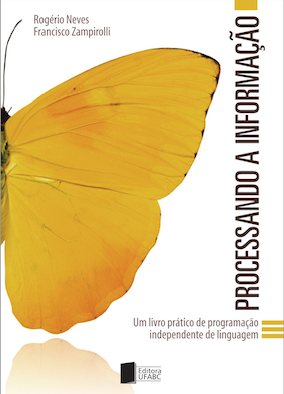
\includegraphics{"figs/Capa_Processando_Informacao.jpg"}

Este caderno (Notebook) é parte complementar \emph{online} do livro
\textbf{\href{https://editora.ufabc.edu.br/matematica-e-ciencias-da-computacao/58-processando-a-informacao}{Processando
a Informação}: um livro prático de programação independente de
linguagem}, que deve ser consultado no caso de dúvidas sobre os temas
apresentados.

\begin{quote}
Este conteúdo pode ser copiado e alterado livremente e foi inspirado
nesse livro.
\end{quote}

    \hypertarget{sumuxe1rio}{%
\subsection{Sumário}\label{sumuxe1rio}}

\begin{itemize}
\tightlist
\item
  Revisão do capítulo anterios
\item
  Quando usar repetições?
\item
  Tipos de estruturas de repetição
\item
  Laços aninhados
\item
  Validação de dados com laços
\item
  Interrupção da execução dos laços
\item
  Recursão
\item
  Revisão deste capítulo
\item
  Exercícios
\end{itemize}

    \hypertarget{revisuxe3o-do-capuxedtulo-anterior-desvios-condicionais}{%
\subsection{Revisão do capítulo anterior (Desvios
Condicionais)}\label{revisuxe3o-do-capuxedtulo-anterior-desvios-condicionais}}

    \begin{itemize}
\item
  No capítulo anterior foram apresentadas formas de construir código
  contendo estruturas condicionais simples ou compostas. Ou seja,
  desvios condicionais, da forma:

  \begin{itemize}
  \tightlist
  \item
    \texttt{se} algo for verdade, \texttt{então}

    \begin{itemize}
    \tightlist
    \item
      faça algo1,
    \end{itemize}
  \item
    \texttt{senão} \# essa parte é opcional

    \begin{itemize}
    \tightlist
    \item
      faça algo2.
    \end{itemize}
  \end{itemize}
\item
  Neste capítulo iremos abordar as \textbf{Estruturas de Repetição},
  conhecidas também como \textbf{Laços} ou \textbf{\emph{Loops}}.
\end{itemize}

    \hypertarget{quando-usar-repetiuxe7uxf5es}{%
\subsection{Quando usar
repetições?}\label{quando-usar-repetiuxe7uxf5es}}

    \begin{itemize}
\item
  As estruturas de repetição são recomendadas para quando um padrão de
  código é repetido várias vezes sequencialmente, apenas alterando-se o
  valor de uma ou mais variáveis entre os comandos repetidos.
\item
  Veja no exemplo a seguir um pseudocodigo, para imprimir a tabuada de
  um número \texttt{t} entrado pelo usuário no formato:
\end{itemize}

Tabuada x (número de 1 a 10) = valor

    \begin{verbatim}
Inteiro: t, n = 1;
t = leia("Qual a tabuada? "); 
escreva(t + " x " + n + " = " + t * n);        n = n + 1; 
escreva(t + " x " + n + " = " + t * n);        n = n + 1; 
escreva(t + " x " + n + " = " + t * n);        n = n + 1; 
escreva(t + " x " + n + " = " + t * n);        n = n + 1; 
escreva(t + " x " + n + " = " + t * n);        n = n + 1; 
escreva(t + " x " + n + " = " + t * n);        n = n + 1; 
escreva(t + " x " + n + " = " + t * n);        n = n + 1; 
escreva(t + " x " + n + " = " + t * n);        n = n + 1; 
escreva(t + " x " + n + " = " + t * n);        n = n + 1; 
escreva(t + " x " + n + " = " + t * n);        n = n + 1; 
\end{verbatim}

    \begin{itemize}
\tightlist
\item
  Embora o código não pareça extenso, é fácil imaginar uma situação onde
  tenhamos que repetir 100, 500, 1000 vezes um mesmo bloco de
  instruções.
\end{itemize}

    \hypertarget{tipos-de-estruturas-de-repetiuxe7uxe3o}{%
\subsection{Tipos de estruturas de
repetição}\label{tipos-de-estruturas-de-repetiuxe7uxe3o}}

    \hypertarget{pseudocuxf3digo}{%
\subsubsection{Pseudocódigo}\label{pseudocuxf3digo}}

    \hypertarget{fauxe7a-enquanto}{%
\paragraph{faça-enquanto}\label{fauxe7a-enquanto}}

\begin{verbatim}
faça { 
  comandos 
} enquanto (condição);
\end{verbatim}

    \hypertarget{enquanto-fauxe7a}{%
\paragraph{enquanto-faça}\label{enquanto-fauxe7a}}

\begin{verbatim}
enquanto (condição) faça { 
  comandos 
}
\end{verbatim}

    \hypertarget{para}{%
\paragraph{para}\label{para}}

\begin{verbatim}
para variável = valor_inicial até valor_final, variável++, faça { 
  comandos 
}
\end{verbatim}

    \hypertarget{para-reverso}{%
\paragraph{para reverso}\label{para-reverso}}

\begin{verbatim}
para variável = valor_final até valor_inicial, variável--, faça { 
  comandos 
}
\end{verbatim}

    \begin{itemize}
\item
  Note que no caso do \texttt{enquanto-faça} é necessário que a condição
  seja verdadeira para que os comandos presentes no bloco de execução
  sejam processados.
\item
  Neste caso, se ao entrar no comando enquanto (\emph{while}) a condição
  do teste for falsa, oposto ao \texttt{faça-enquanto}, o subprograma
  não será executado.
\item
  Isto é, todo o código dentro do bloco do laço será pulado já na
  verificação inicial da condição no \texttt{enquanto-faça}, seguindo
  diretamente para a parte sequencial subsequente, similar ao que ocorre
  no se-então.
\item
  A forma \texttt{faça-enquanto} é recomendada quando queremos que os
  comandos contidos no laço sejam executados ao menos uma vez, mesmo que
  a condição seja inicialmente falsa.
\item
  O laço \texttt{para} é recomendado quando se sabe o número de
  iterações existes (quantas vezes o bloco dentro do laço será
  executado). Por exempo, no caso anterior do problema da Tabuada.
\end{itemize}

    \hypertarget{ccppjavajavascript}{%
\subsubsection{C/CPP/Java/JavaScript}\label{ccppjavajavascript}}

    \hypertarget{do-while}{%
\paragraph{do-while}\label{do-while}}

    \begin{verbatim}
do { 
  comandos;
} while (condição);
\end{verbatim}

    \hypertarget{while}{%
\paragraph{while}\label{while}}

    \begin{verbatim}
while (condição) { 
  comandos;
}
\end{verbatim}

    \hypertarget{for}{%
\paragraph{for}\label{for}}

    \begin{verbatim}
for(v=0; v<10; v++) {
  comandos;
}
\end{verbatim}

Em algumas linguagens de programação é possível omitir um ou todos os
parâmetros, por exemplo: \texttt{for(;;)\ \{...\}}.

    \hypertarget{pseudocuxf3digo-exemplo-lauxe7o-fauxe7a-enquanto.}{%
\subsubsection{Pseudocódigo: Exemplo laço
faça-enquanto.}\label{pseudocuxf3digo-exemplo-lauxe7o-fauxe7a-enquanto.}}

\begin{verbatim}
Real: nota, média, acumulador=0, contador=0;
Caractere: resposta='lixo';

faça {
   nota = leia("Entre com uma nota: ");
   acumulador = acumulador + nota;
   contador = contador + 1;
   resposta = leia("Deseja continuar? (s/n): ");
} enquanto (resposta == 's');

média = acumulador / contador;
imprima ("A média das " + contador + " notas é " + média);
\end{verbatim}

    \begin{itemize}
\item
  Além do \texttt{contador}, o programa usa um \texttt{acumulador}
  (variável que acumula as notas digitadas).
\item
  Repare que a condição
  \texttt{resposta\ ==\ \textquotesingle{}s\textquotesingle{}} no
  \texttt{faça-enquanto} é falsa até que seja efetuada a leitura da
  variável resposta dentro do laço, em:
  \texttt{resposta\ =\ leia("Deseja\ continuar?\ (s/n):\ ");}
\item
  Apenas do caso de o usuário entrar com o caractere
  \texttt{\textquotesingle{}s\textquotesingle{}}, o laço será repetido
  novamente.
\item
  Isto quer dizer que o estado da condição é falso na primeira execução
  do código do laço.
\end{itemize}

    \hypertarget{pseudocuxf3digo-exemplo-lauxe7o-enquanto-fauxe7a.}{%
\subsubsection{Pseudocódigo: Exemplo laço
enquanto-faça.}\label{pseudocuxf3digo-exemplo-lauxe7o-enquanto-fauxe7a.}}

\begin{verbatim}
Real: nota, média, acumulador=0, contador=0;
Caractere: resposta='s';

enquanto (resposta == 's') faça {
   nota = leia("Entre com uma nota: ");
   acumulador = acumulador + nota;
   contador = contador + 1;
   resposta = leia("Deseja continuar? (s/n): ");
} 

média = acumulador / contador;
imprima ("A média das " + contador + " notas é " + média);
\end{verbatim}

    \begin{itemize}
\tightlist
\item
  Observe que no pseudocódigo anterior do \texttt{enquanto-faça} temos o
  mesmo resultado do \texttt{faça-enquanto}, pois a variável
  \texttt{resposta} é inicializada com \texttt{s}, satisfazendo a
  condição lógica e entrando no laço.
\end{itemize}

    \begin{itemize}
\tightlist
\item
  Ver Fluxograma abaixo (também experimente nessa ferramenta
  \emph{online}: \href{https://app.code2flow.com/}{code2flow}, copiando
  e colando o código em vermelho abaixo):
\end{itemize}

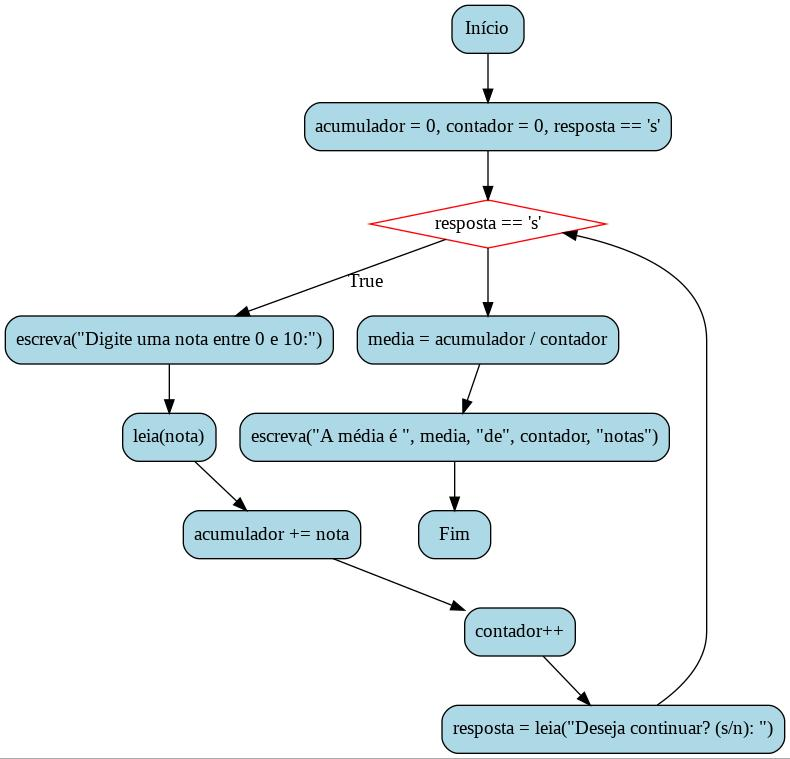
\includegraphics{"figs/flowchartCap4a.png"}

    \begin{figure}
\centering
\caption{flowchartCap4a.png}
\end{figure}

    \begin{tcolorbox}[breakable, size=fbox, boxrule=1pt, pad at break*=1mm,colback=cellbackground, colframe=cellborder]
\prompt{In}{incolor}{ }{\boxspacing}
\begin{Verbatim}[commandchars=\\\{\}]
\PY{o}{!}apt\PYZhy{}get install graphviz libgraphviz\PYZhy{}dev pkg\PYZhy{}config
\PY{o}{!}pip install txtoflow
\end{Verbatim}
\end{tcolorbox}

    \begin{tcolorbox}[breakable, size=fbox, boxrule=1pt, pad at break*=1mm,colback=cellbackground, colframe=cellborder]
\prompt{In}{incolor}{ }{\boxspacing}
\begin{Verbatim}[commandchars=\\\{\}]
\PY{k+kn}{from} \PY{n+nn}{txtoflow} \PY{k+kn}{import} \PY{n}{txtoflow}

\PY{n}{txtoflow}\PY{o}{.}\PY{n}{generate}\PY{p}{(}
    \PY{l+s+sd}{\PYZsq{}\PYZsq{}\PYZsq{}}
\PY{l+s+sd}{    Início;}
\PY{l+s+sd}{    acumulador = 0, contador = 0, resposta == \PYZsq{}s\PYZsq{};}
\PY{l+s+sd}{    while (resposta == \PYZsq{}s\PYZsq{}) \PYZob{}}
\PY{l+s+sd}{      escreva(\PYZdq{}Digite uma nota entre 0 e 10:\PYZdq{});}
\PY{l+s+sd}{      leia(nota);}
\PY{l+s+sd}{      acumulador += nota;}
\PY{l+s+sd}{      contador++;}
\PY{l+s+sd}{      resposta = leia(\PYZdq{}Deseja continuar? (s/n): \PYZdq{});}
\PY{l+s+sd}{    \PYZcb{}}
\PY{l+s+sd}{    media = acumulador / contador;}
\PY{l+s+sd}{    escreva(\PYZdq{}A média é \PYZdq{}, media, \PYZdq{}de\PYZdq{}, contador, \PYZdq{}notas\PYZdq{});}
\PY{l+s+sd}{    Fim;}
\PY{l+s+sd}{    \PYZsq{}\PYZsq{}\PYZsq{}}
\PY{p}{)}
\end{Verbatim}
\end{tcolorbox}

    \hypertarget{pseudocuxf3digo-exemplo-lauxe7o-enquanto-fauxe7a-infinito.}{%
\subsubsection{Pseudocódigo: Exemplo laço enquanto-faça
INFINITO.}\label{pseudocuxf3digo-exemplo-lauxe7o-enquanto-fauxe7a-infinito.}}

Considere uma alteração no código anterior para não fazer mais a
pergunta \texttt{Deseja\ continuar?\ (s/n)}, mas entrando num laço
\texttt{enquanto-faça} para ler e acumular 100 notas:

\begin{verbatim}
Real: nota, média, acumulador=0,contador=0;

enquanto (contador < 100) faça {
   nota = leia("Entre com uma nota: ");
   acumulador = acumulador + nota;
   # contador = contador + 1;
} 

média = acumulador / contador;
imprima ("A média das " + contador + " notas é " + média);
\end{verbatim}

    \begin{itemize}
\tightlist
\item
  O que vai ocorrer ao escrever e rodar esse código em alguma linguagem
  de programação?
\item
  Onde está o erro?
\item
  \textbf{MUITO CUIDADO COM LAÇOS INFINITOS EM ATIVIDADES NO
  MOODLE+VPL!} Se a execução demorar mais que 1 minuto, provavelmente
  entrou em um laço infinito e terá que recarregar a página.
\item
  Esta condição, onde a execução fica ``presa'' dentro do laço, é
  conhecida como \textbf{\emph{DEADLOCK}}.
\item
  \emph{Deadlocks} geram erro de finalização de programa, que executará
  eternamente, podendo travar o programa, o teclado e o mouse ou até
  mesmo o computador, neste caso, sendo necessário um
  \textbf{\emph{RESET}} para sair do laço.
\end{itemize}

    \hypertarget{validauxe7uxe3o-de-dados}{%
\subsection{Validação de Dados}\label{validauxe7uxe3o-de-dados}}

    \begin{itemize}
\item
  Uma possível aplicação de laços é garantir que os dados entrados sejam
  válidos.
\item
  \textbf{Validação de dados} é o nome dado à verificação dos valores de
  entrada, se os mesmos se encontram dentro dos limites previstos ou no
  formato adequado, notificando o usuário no caso de valores inválidos.
\item
  O exemplo a seguir é o pseudocódigo apresentado anteriormente,
  incorporando a validação de dados de entrada (nota entre 0 e 10),
  indicando o erro e pedindo para o usuário entrar novamente o dado até
  que seja válido.
\end{itemize}

    \hypertarget{pseudocuxf3digo-exemplo-lauxe7o-fauxe7a-enquanto-com-validauxe7uxe3o}{%
\subsubsection{Pseudocódigo: Exemplo laço faça-enquanto, com
validação}\label{pseudocuxf3digo-exemplo-lauxe7o-fauxe7a-enquanto-com-validauxe7uxe3o}}

\begin{verbatim}
Real: nota, média, acumulador=0, contador=0;
Caractere: resposta='lixo';

faça {
  faça {
    nota = leia("Entre com uma nota entre 0 e 10: ");
    se (nota < 0 || nota > 10) então 
      escreva("ERRO, nota inválida. Digital nota entre 0 e 10!")
  } enquanto (nota < 0 || nota > 10); 
  acumulador = acumulador + nota;
  contador = contador + 1;
  resposta = leia("Deseja continuar? (s/n): ");
} enquanto (resposta == 's');

média = acumulador / contador;
imprima ("A média das " + contador + " notas é " + média);
\end{verbatim}

    \begin{itemize}
\tightlist
\item
  No pseudocódigo anterior, o segundo \texttt{faça-enquanto} aceita
  apenas notas entre 0 e 10. Caso contrário, escreve uma mensagem de
  erro e solicita nova nota.
\end{itemize}

    \begin{itemize}
\item
  Ver Fluxograma abaixo (também experimente nessa ferramenta
  \emph{online}: \href{https://app.code2flow.com/}{code2flow}, copiando
  e colando o código em vermelho abaixo).
\item
  Observar que essa biblioteca \texttt{txtoflow} não aceita
  \texttt{faça-enquanto}, assim como o Python.
\end{itemize}

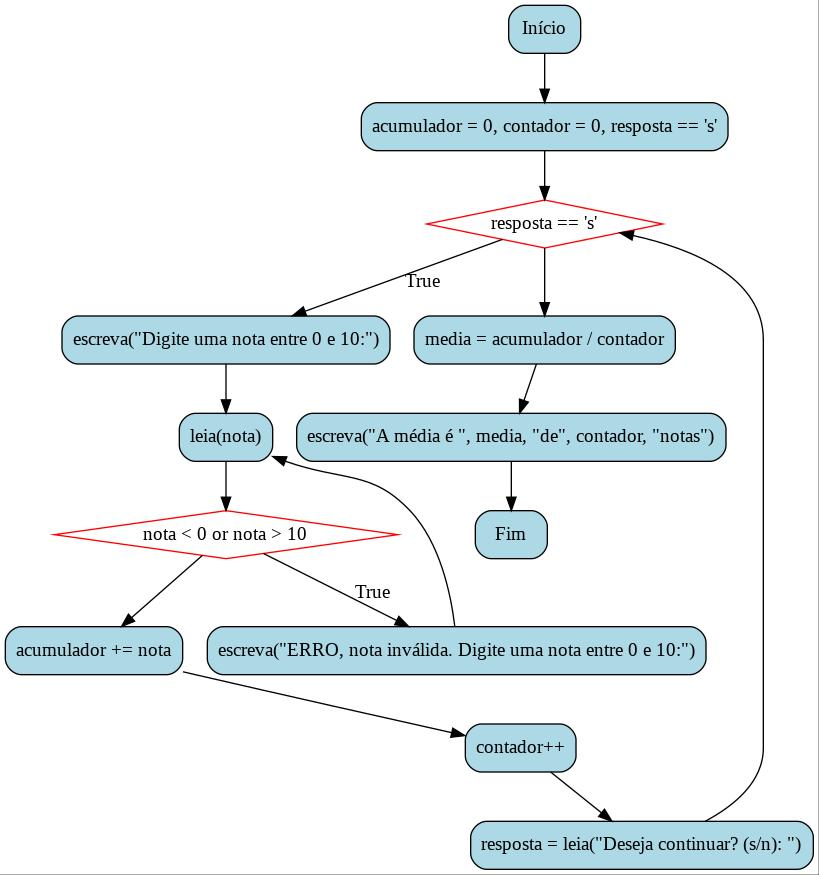
\includegraphics{"figs/flowchartCap4b.png"}

    \begin{figure}
\centering
\caption{flowchartCap4b.png}
\end{figure}

    \begin{tcolorbox}[breakable, size=fbox, boxrule=1pt, pad at break*=1mm,colback=cellbackground, colframe=cellborder]
\prompt{In}{incolor}{ }{\boxspacing}
\begin{Verbatim}[commandchars=\\\{\}]
\PY{o}{!}apt\PYZhy{}get install graphviz libgraphviz\PYZhy{}dev pkg\PYZhy{}config
\PY{o}{!}pip install txtoflow
\end{Verbatim}
\end{tcolorbox}

    \begin{tcolorbox}[breakable, size=fbox, boxrule=1pt, pad at break*=1mm,colback=cellbackground, colframe=cellborder]
\prompt{In}{incolor}{ }{\boxspacing}
\begin{Verbatim}[commandchars=\\\{\}]
\PY{k+kn}{from} \PY{n+nn}{txtoflow} \PY{k+kn}{import} \PY{n}{txtoflow}

\PY{n}{txtoflow}\PY{o}{.}\PY{n}{generate}\PY{p}{(}
    \PY{l+s+sd}{\PYZsq{}\PYZsq{}\PYZsq{}}
\PY{l+s+sd}{    Início;}
\PY{l+s+sd}{    acumulador = 0, contador = 0, resposta == \PYZsq{}s\PYZsq{};}
\PY{l+s+sd}{    while (resposta == \PYZsq{}s\PYZsq{}) \PYZob{}}
\PY{l+s+sd}{      escreva(\PYZdq{}Digite uma nota entre 0 e 10:\PYZdq{});}
\PY{l+s+sd}{      leia(nota);}
\PY{l+s+sd}{      while (nota \PYZlt{} 0 or nota \PYZgt{} 10) \PYZob{}}
\PY{l+s+sd}{        escreva(\PYZdq{}ERRO, nota inválida. Digite uma nota entre 0 e 10:\PYZdq{});}
\PY{l+s+sd}{        leia(nota);}
\PY{l+s+sd}{      \PYZcb{}}
\PY{l+s+sd}{      acumulador += nota;}
\PY{l+s+sd}{      contador++;}
\PY{l+s+sd}{      resposta = leia(\PYZdq{}Deseja continuar? (s/n): \PYZdq{});}
\PY{l+s+sd}{    \PYZcb{}}
\PY{l+s+sd}{    media = acumulador / contador;}
\PY{l+s+sd}{    escreva(\PYZdq{}A média é \PYZdq{}, media, \PYZdq{}de\PYZdq{}, contador, \PYZdq{}notas\PYZdq{});}
\PY{l+s+sd}{    Fim;}
\PY{l+s+sd}{    \PYZsq{}\PYZsq{}\PYZsq{}}
\PY{p}{)}
\end{Verbatim}
\end{tcolorbox}

    \hypertarget{interrupuxe7uxe3o-dos-lauxe7os}{%
\subsection{Interrupção dos
laços}\label{interrupuxe7uxe3o-dos-lauxe7os}}

    \begin{itemize}
\item
  Algumas linguagens permitem interromper a execução do laço através do
  comando `interromper' ou `quebrar' (\textbf{break}).
\item
  Isto pode ser útil caso se queira interromper o laço em algum evento
  específico.
\end{itemize}

    \hypertarget{exemplo-01---ler-10-notas-com-validauxe7uxe3o}{%
\subsection{Exemplo 01 - Ler 10 notas com
validação}\label{exemplo-01---ler-10-notas-com-validauxe7uxe3o}}

Considere um algoritmo para ler 10 notas válidas, entre 0 e 10,
escrevendo no final a média nas notas válidas lidas.

    Pseudocódigo

\begin{verbatim}
Real: nota, média, acumulador=0,contador=0;

escreva("Entre com 10 notas válidas")
faça {
  faça {
    nota = leia();
  } enquanto (nota < 0 || nota > 10); 
  acumulador = acumulador + nota;
  contador = contador + 1;
} enquanto (contador < 10);

média = acumulador / contador;
escreva("A média das " + contador + " notas é " + média);
\end{verbatim}

    \begin{itemize}
\tightlist
\item
  Ver Fluxograma abaixo (também experimente nessa ferramenta
  \emph{online}: \href{https://app.code2flow.com/}{code2flow}, copiando
  e colando o código em vermelho abaixo):
\end{itemize}

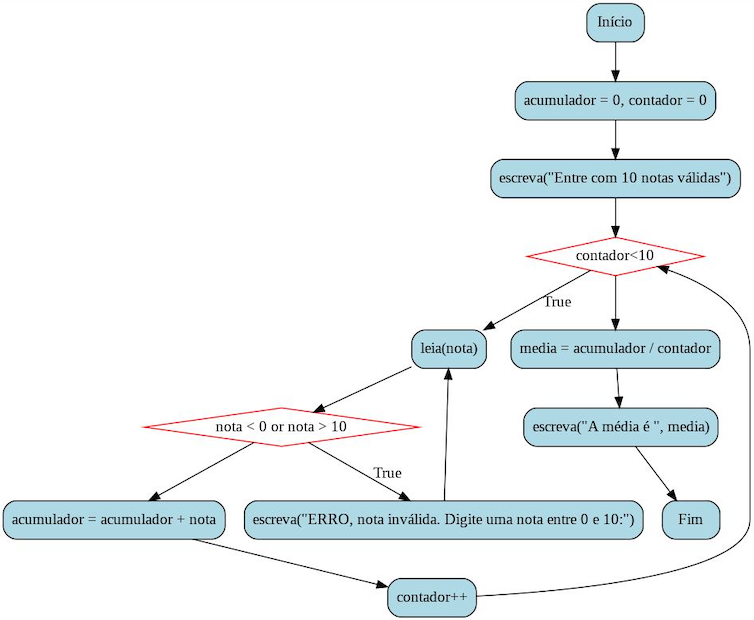
\includegraphics{"figs/flowchartCap4c.png"}

    \begin{figure}
\centering
\caption{flowchartCap4c.jpg}
\end{figure}

    \begin{tcolorbox}[breakable, size=fbox, boxrule=1pt, pad at break*=1mm,colback=cellbackground, colframe=cellborder]
\prompt{In}{incolor}{ }{\boxspacing}
\begin{Verbatim}[commandchars=\\\{\}]
\PY{o}{!}apt\PYZhy{}get install graphviz libgraphviz\PYZhy{}dev pkg\PYZhy{}config
\PY{o}{!}pip install txtoflow
\end{Verbatim}
\end{tcolorbox}

    \begin{tcolorbox}[breakable, size=fbox, boxrule=1pt, pad at break*=1mm,colback=cellbackground, colframe=cellborder]
\prompt{In}{incolor}{ }{\boxspacing}
\begin{Verbatim}[commandchars=\\\{\}]
\PY{k+kn}{from} \PY{n+nn}{txtoflow} \PY{k+kn}{import} \PY{n}{txtoflow}

\PY{n}{txtoflow}\PY{o}{.}\PY{n}{generate}\PY{p}{(}
    \PY{l+s+sd}{\PYZsq{}\PYZsq{}\PYZsq{}}
\PY{l+s+sd}{    Início;}
\PY{l+s+sd}{    acumulador = 0, contador = 0;}
\PY{l+s+sd}{    escreva(\PYZdq{}Entre com 10 notas válidas\PYZdq{});}
\PY{l+s+sd}{    while (contador\PYZlt{}10) \PYZob{}}
\PY{l+s+sd}{      leia(nota);}
\PY{l+s+sd}{      while (nota \PYZlt{} 0 or nota \PYZgt{} 10) \PYZob{}}
\PY{l+s+sd}{        escreva(\PYZdq{}ERRO, nota inválida. Digite uma nota entre 0 e 10:\PYZdq{});}
\PY{l+s+sd}{        leia(nota);}
\PY{l+s+sd}{      \PYZcb{}}
\PY{l+s+sd}{      acumulador = acumulador + nota;}
\PY{l+s+sd}{      contador++;}
\PY{l+s+sd}{    \PYZcb{}}
\PY{l+s+sd}{    media = acumulador / contador;}
\PY{l+s+sd}{    escreva(\PYZdq{}A média é \PYZdq{}, media);}
\PY{l+s+sd}{    Fim;}
\PY{l+s+sd}{    \PYZsq{}\PYZsq{}\PYZsq{}}
\PY{p}{)}
\end{Verbatim}
\end{tcolorbox}

    Casos para Teste Moodle+VPL

Para o professor criar uma atividade VPL no Moodle para este Exemplo 01,
basta incluir em \texttt{Casos\ para\ teste}, o seguinte texto (pode
incluir mais casos):

\begin{verbatim}
case=caso1
input=9.0
78.0
6.0
9
8
7
6
5
7
8
6
output= 
A média das 10 notas é 7.1
case=caso2
input=9.0
78.0
-9.0
9876.0
9876.0
7.0
9
8
4
6
6
8
9
7
output= 
A média das 10 notas é 7.3
\end{verbatim}

    \begin{tcolorbox}[breakable, size=fbox, boxrule=1pt, pad at break*=1mm,colback=cellbackground, colframe=cellborder]
\prompt{In}{incolor}{1}{\boxspacing}
\begin{Verbatim}[commandchars=\\\{\}]
\PY{o}{\PYZpc{}\PYZpc{}writefile} cap4ex01.c
\PY{c+c1}{\PYZsh{}include \PYZlt{}stdio.h\PYZgt{}}

\PY{n+nb}{int} \PY{n}{main}\PY{p}{(}\PY{n}{void}\PY{p}{)} \PY{p}{\PYZob{}}

  \PY{o}{/}\PY{o}{/} \PY{n}{ENTRADA} \PY{n}{DE} \PY{n}{DADOS} \PY{n}{e} \PY{n}{PROCESSAMENTO}
  \PY{n+nb}{float} \PY{n}{acumulador} \PY{o}{=} \PY{l+m+mi}{0}\PY{p}{,} \PY{n}{nota}\PY{p}{,} \PY{n}{media}\PY{p}{;}
  \PY{n+nb}{int} \PY{n}{contador} \PY{o}{=} \PY{l+m+mi}{0}\PY{p}{;}
  
  \PY{n}{printf}\PY{p}{(}\PY{l+s+s2}{\PYZdq{}}\PY{l+s+s2}{Entre com 10 notas válidas}\PY{l+s+se}{\PYZbs{}n}\PY{l+s+s2}{\PYZdq{}}\PY{p}{)}\PY{p}{;}
  \PY{k}{while} \PY{p}{(}\PY{n}{contador}\PY{o}{\PYZlt{}}\PY{l+m+mi}{10}\PY{p}{)} \PY{p}{\PYZob{}}
    \PY{n}{do} \PY{p}{\PYZob{}}
        \PY{n}{scanf}\PY{p}{(}\PY{l+s+s2}{\PYZdq{}}\PY{l+s+si}{\PYZpc{}f}\PY{l+s+s2}{\PYZdq{}}\PY{p}{,} \PY{o}{\PYZam{}}\PY{n}{nota}\PY{p}{)}\PY{p}{;}
    \PY{p}{\PYZcb{}} \PY{k}{while} \PY{p}{(}\PY{n}{nota} \PY{o}{\PYZlt{}} \PY{l+m+mf}{0.0} \PY{o}{|}\PY{o}{|} \PY{n}{nota} \PY{o}{\PYZgt{}} \PY{l+m+mf}{10.0} \PY{p}{)}\PY{p}{;}
    \PY{n}{acumulador} \PY{o}{=} \PY{n}{acumulador} \PY{o}{+} \PY{n}{nota}\PY{p}{;}
    \PY{n}{contador}\PY{o}{+}\PY{o}{+}\PY{p}{;}
  \PY{p}{\PYZcb{}}
  \PY{n}{media} \PY{o}{=} \PY{n}{acumulador}\PY{o}{/}\PY{n}{contador}\PY{p}{;}

  \PY{o}{/}\PY{o}{/} \PY{n}{SAÍDA}
  \PY{n}{printf}\PY{p}{(}\PY{l+s+s2}{\PYZdq{}}\PY{l+s+s2}{A média das }\PY{l+s+si}{\PYZpc{}d}\PY{l+s+s2}{ notas é }\PY{l+s+si}{\PYZpc{}.1f}\PY{l+s+se}{\PYZbs{}n}\PY{l+s+s2}{\PYZdq{}}\PY{p}{,} \PY{n}{contador}\PY{p}{,} \PY{n}{media}\PY{p}{)}\PY{p}{;}

  \PY{k}{return} \PY{l+m+mi}{0}\PY{p}{;}
\PY{p}{\PYZcb{}}
\end{Verbatim}
\end{tcolorbox}

    \begin{tcolorbox}[breakable, size=fbox, boxrule=1pt, pad at break*=1mm,colback=cellbackground, colframe=cellborder]
\prompt{In}{incolor}{2}{\boxspacing}
\begin{Verbatim}[commandchars=\\\{\}]
\PY{o}{\PYZpc{}\PYZpc{}}\PY{k}{shell}
gcc \PYZhy{}Wall \PYZhy{}std=c99 cap4ex01.c \PYZhy{}o output2
./output2
\end{Verbatim}
\end{tcolorbox}

    \hypertarget{recursuxe3o}{%
\subsection{Recursão}\label{recursuxe3o}}

    Este tópico de recursão (ou recursividade) é complementar ao livro, eu
sua primeira edição.

Como nos laços de repetição, a recursão tem como objetivo rodar trechos
de códigos (agora encapsulados em métodos) várias vezes.

Além disso, análogo ao laço, \textbf{muito cuidado com o critério de
parada, senão o código irá fazer infinitas chamadas recursivas, podendo
travar o seu computador!}

Ou seja, o método recursivo teve ter pelo menos uma condicional e
argumentos que variam nas chamadas recursivas. Veja um exemplo a seguir.

    \hypertarget{exemplo-02---ler-10-notas-com-recursuxe3o}{%
\subsection{Exemplo 02 - Ler 10 notas, com
recursão}\label{exemplo-02---ler-10-notas-com-recursuxe3o}}

Considere um algoritmo para ler 10 notas válidas utilizando recursão e
calcular a média.

    Pseudocódigo

\begin{verbatim}
# MINHA FUNÇÃO RECURSIVA
função lerNota(recebe: real acumulador, inteiro n) retorna real acumulador {
  Real: nota;
  se (n > 0) faça { # CRITÉRIO DE PARADA
    faça {
      nota = leia();
    } enquanto (nota < 0 || nota > 10); 
    acumulador = lerNota(acumulador, n - 1); # CHAMADA RECURSIVA, 
    # COM ALTERAÇÃO DO VALOR DO ARGUMENTO !!!
  }
  retorne acumulador + nota;
}

Real: média, acumulador=0, contador=10;

escreva("Entre com " + contador + " notas válidas")
acumulador = lerNota(acumulador, contador); # CHAMDADA RECURSIVA!!!

média = acumulador / contador;
escreva("A média das " + contador + " notas é " + média);
\end{verbatim}

    \begin{tcolorbox}[breakable, size=fbox, boxrule=1pt, pad at break*=1mm,colback=cellbackground, colframe=cellborder]
\prompt{In}{incolor}{5}{\boxspacing}
\begin{Verbatim}[commandchars=\\\{\}]
\PY{o}{\PYZpc{}\PYZpc{}writefile} cap4ex02.c
\PY{c+c1}{\PYZsh{}include \PYZlt{}stdio.h\PYZgt{}}

\PY{n+nb}{float} \PY{n}{lerNota}\PY{p}{(}\PY{n+nb}{float} \PY{n}{acumulador}\PY{p}{,} \PY{n+nb}{int} \PY{n}{n}\PY{p}{)} \PY{p}{\PYZob{}}
  \PY{n+nb}{float} \PY{n}{nota}\PY{p}{;}
  \PY{k}{if} \PY{p}{(}\PY{n}{n} \PY{o}{\PYZgt{}} \PY{l+m+mi}{0}\PY{p}{)} \PY{p}{\PYZob{}} \PY{o}{/}\PY{o}{/} \PY{n}{CRITÉRIO} \PY{n}{DE} \PY{n}{PARADA}
    \PY{n}{do} \PY{p}{\PYZob{}}
      \PY{n}{scanf}\PY{p}{(}\PY{l+s+s2}{\PYZdq{}}\PY{l+s+si}{\PYZpc{}f}\PY{l+s+s2}{\PYZdq{}}\PY{p}{,} \PY{o}{\PYZam{}}\PY{n}{nota}\PY{p}{)}\PY{p}{;}
    \PY{p}{\PYZcb{}} \PY{k}{while} \PY{p}{(}\PY{n}{nota} \PY{o}{\PYZlt{}} \PY{l+m+mf}{0.0} \PY{o}{|}\PY{o}{|} \PY{n}{nota} \PY{o}{\PYZgt{}} \PY{l+m+mf}{10.0}\PY{p}{)}\PY{p}{;}
    \PY{n}{acumulador} \PY{o}{=} \PY{n}{lerNota}\PY{p}{(}\PY{n}{acumulador}\PY{p}{,} \PY{n}{n} \PY{o}{\PYZhy{}} \PY{l+m+mi}{1}\PY{p}{)}\PY{p}{;} \PY{o}{/}\PY{o}{/} \PY{n}{CHAMADA} \PY{n}{RECURSIVA}\PY{p}{,} 
    \PY{o}{/}\PY{o}{/} \PY{n}{COM} \PY{n}{ALTERAÇÃO} \PY{n}{DO} \PY{n}{VALOR} \PY{n}{DO} \PY{n}{ARGUMENTO} \PY{err}{!}\PY{err}{!}\PY{err}{!}
  \PY{p}{\PYZcb{}}
  \PY{k}{return} \PY{n}{acumulador} \PY{o}{+} \PY{n}{nota}\PY{p}{;}
\PY{p}{\PYZcb{}}

\PY{n+nb}{int} \PY{n}{main}\PY{p}{(}\PY{n}{void}\PY{p}{)} \PY{p}{\PYZob{}}

  \PY{o}{/}\PY{o}{/} \PY{n}{ENTRADA} \PY{n}{DE} \PY{n}{DADOS} \PY{n}{e} \PY{n}{PROCESSAMENTO}
  \PY{n+nb}{float} \PY{n}{acumulador} \PY{o}{=} \PY{l+m+mi}{0}\PY{p}{,} \PY{n}{media}\PY{p}{;}
  \PY{n+nb}{int} \PY{n}{contador} \PY{o}{=} \PY{l+m+mi}{10}\PY{p}{;}

  \PY{n}{printf}\PY{p}{(}\PY{l+s+s2}{\PYZdq{}}\PY{l+s+s2}{Entre com }\PY{l+s+si}{\PYZpc{}d}\PY{l+s+s2}{ notas válidas}\PY{l+s+se}{\PYZbs{}n}\PY{l+s+s2}{\PYZdq{}}\PY{p}{,} \PY{n}{contador}\PY{p}{)}\PY{p}{;}
  \PY{n}{acumulador} \PY{o}{=} \PY{n}{lerNota}\PY{p}{(}\PY{n}{acumulador}\PY{p}{,} \PY{n}{contador}\PY{p}{)}\PY{p}{;}
  \PY{n}{media} \PY{o}{=} \PY{n}{acumulador} \PY{o}{/} \PY{n}{contador}\PY{p}{;}

  \PY{o}{/}\PY{o}{/} \PY{n}{SAÍDA}
  \PY{n}{printf}\PY{p}{(}\PY{l+s+s2}{\PYZdq{}}\PY{l+s+s2}{A média das }\PY{l+s+si}{\PYZpc{}d}\PY{l+s+s2}{ notas é }\PY{l+s+si}{\PYZpc{}.1f}\PY{l+s+se}{\PYZbs{}n}\PY{l+s+s2}{\PYZdq{}}\PY{p}{,} \PY{n}{contador}\PY{p}{,} \PY{n}{media}\PY{p}{)}\PY{p}{;}

  \PY{k}{return} \PY{l+m+mi}{0}\PY{p}{;}
\PY{p}{\PYZcb{}}
\end{Verbatim}
\end{tcolorbox}

    \begin{tcolorbox}[breakable, size=fbox, boxrule=1pt, pad at break*=1mm,colback=cellbackground, colframe=cellborder]
\prompt{In}{incolor}{6}{\boxspacing}
\begin{Verbatim}[commandchars=\\\{\}]
\PY{o}{\PYZpc{}\PYZpc{}}\PY{k}{shell}
gcc \PYZhy{}Wall \PYZhy{}std=c99 cap4ex02.c \PYZhy{}o output2
./output2
\end{Verbatim}
\end{tcolorbox}

    \hypertarget{exercuxedcios}{%
\subsection{Exercícios}\label{exercuxedcios}}

    Ver notebook Colab no arquivo \texttt{cap4.part2.lab.*.ipynb}
(\texttt{*} é a extensão da linguagem), utilizando alguma linguagem de
programação de sua preferência, onganizadas em subpastas contidas de
\texttt{"gen"}, na pasta do Google Drive
\href{https://drive.google.com/drive/folders/1YlFwv8XYN7PYYf-HwDMlkxzbmXzJw9cM?usp=sharing}{colabs}.

    \hypertarget{revisuxe3o-deste-capuxedtulo-de-estruturas-de-repetiuxe7uxe3o-lauxe7os}{%
\subsection{Revisão deste capítulo de Estruturas de Repetição
(Laços)}\label{revisuxe3o-deste-capuxedtulo-de-estruturas-de-repetiuxe7uxe3o-lauxe7os}}

\begin{itemize}
\tightlist
\item
  Quando usar repetições? \textgreater{} Quando existem instruções que
  se repentem.
\item
  Tipos de estruturas de repetição:

  \begin{itemize}
  \tightlist
  \item
    Depende da linguagem. Algumas possibilidades:

    \begin{itemize}
    \tightlist
    \item
      \texttt{do-while} (não aceita em Python)
    \item
      \texttt{while} (todas)
    \item
      \texttt{for} (todas)
    \item
      \texttt{repeat} (R)
    \end{itemize}
  \item
    Qual usar?

    \begin{itemize}
    \tightlist
    \item
      Depende da lógica ser implementada e da linguagem utilizada.
    \item
      Se tiver um número fixo de iterações, geralmente se usa
      \texttt{for}.
    \end{itemize}
  \end{itemize}
\item
  Laços aninhados
\item
  Validação de dados com laços

  \begin{itemize}
  \tightlist
  \item
    Incluir um laço para verificar o valor lido.
  \end{itemize}
\item
  Interrupção da execução dos laços

  \begin{itemize}
  \tightlist
  \item
    Depende da linguagem, algumas possibilidades:

    \begin{itemize}
    \tightlist
    \item
      \texttt{break} - interrompe o laço
    \item
      \texttt{continue} - não executa o final do laço
    \item
      \texttt{exit} - aborta o laço e o programa!
    \end{itemize}
  \end{itemize}
\item
  Outra forma de executar trechos de códigos várias vezes é encapsular
  em métodos recursivos.

  \begin{itemize}
  \tightlist
  \item
    Atenção com o critério de parada!
  \item
    Atenção com os argumentos do método recursivo!
  \end{itemize}
\item
  Exercícios
\item
  Revisão deste capítulo de Estruturas de Repetição (Laços)
\end{itemize}


    % Add a bibliography block to the postdoc
    
    
    
\end{document}
